\documentclass[gr-notes.tex]{subfiles}

\begin{document}

\setcounter{chapter}{0}

\chapter{Special relativity}

\section{Fundamental principles of special relativity (SR) theory}

Special relativity can be summarized by two fundamental postulates:


\begin{enumerate}
\item The principle of relativity (Galileo), which states that no experiment
  may measure the absolute velocity of an observer.
\item The universality of the speed of light (Einstein), which states that
  the speed of light is constant when measured from any inertial reference
  frame.
\end{enumerate}


\section{Definition of an inertial observer in SR}

When we say ``observer'', what we really mean is a coordinate system. Thus an inertial observer is a coordinate system that meets the following 3 criteria:

\begin{enumerate}
\item The distance between two spatial points $P_1$ and $P_2$ is independent of
  time.
\item Time is synchronized and moves at the same rate at all spatial points.
\item At any constant time, space is Euclidean.
\end{enumerate}

It follows from these criteria that the observer must be \textbf{unaccelerated}.

\section{New units}

The speed of light, $c$, is approximately $\SI{3.00e8}{\meter\second^{-1}}$ in SI units. However, these units predate relativity, and are very inconvenient. Life becomes easier if we define our units around $c$, such that $c \equiv 1$.

This can be done by repurposing the meter as a measure of time as well. We thereby define the meter as ``the time it takes light to travel 1 meter''. Thus the speed of light becomes

\begin{displaymath}
  c = \frac{\SI{1}{\meter}}{\SI{1}{\meter}}.
\end{displaymath}

Indeed, it turns out in SR that time is most conveniently measured in distance ($c = \SI{3.00e10}{\centi\meter}$), and in GR mass is as well ($G/c^{-2} = \SI{7.425e-29}{\centi\meter\per\gram}$).


\section{Spacetime diagrams}

\section{Construction of the coordinates used by another observer}

\section{Invariance of the interval}

For two nearby events, we can define the \textbf{invariant interval}, defining a 4D Minskowski spacetime:

\begin{displaymath}
  \dd{s}^2 = -(c \dd{t})^2 + \dd{x}^2 + \dd{y}^2 + \dd{z}^2,
\end{displaymath}

or when we set $c \equiv 1$:

\begin{displaymath}
  \dd{s}^2 = -\dd{t}^2 + \dd{x}^2 + \dd{y}^2 + \dd{z}^2.
%
  \tag{Schutz 1.1}
  \label{schutz:1.1}
\end{displaymath}

This notation can be simplified be defining

\begin{displaymath}
  \eta_{\mu\nu} =
  \diag(-1, 1, 1, 1) =
  \mqty(-1 & 0 & 0 & 0 \\
         0 & 1 & 0 & 0 \\
         0 & 0 & 1 & 0 \\
         0 & 0 & 0 & 1);
  \quad
  \dd{s}^2 = \sum_{\mu=0}^3 \sum_{\nu=0}^3 \eta_{\mu\nu} \dd{x}^\mu \dd{x}^\nu
\end{displaymath}

When we want to find $\dd{\bar{s}}^2$, we can consider the fact that each of its components, $\dd{\bar{x}^\alpha}$, is a linear combination of the components of $\dd{s}^2$,
%
\begin{displaymath}
  \dd{\bar{x}^\alpha} = \sum_{\beta=0}^3 a_{\alpha\beta} x^\beta.
\end{displaymath}
%
Now, when we consider the square of $\dd{\bar{x}^\alpha}$, the cross terms make it a quadratic function. Since the sum of four quadratics (the four $\dd{\bar{x}^\alpha}$'s) is also a quadratic, we can write $\dd{\bar{s}}^2$ as
%
\begin{displaymath}
  \dd{\bar{s}} =
  \sum_{\alpha=0}^3 \sum_{\beta=0}^3
      M_{\alpha\beta} (\dd{x^\alpha}) (\dd{x^\beta})
%
  \tag{Schutz 1.2}
  \label{schutz:1.2}
\end{displaymath}
%
If are talking about light, $\dd{s}^2 = 0$, and so we can say
%
\begin{displaymath}
  \dd{s}^2 = 0 = -\dd{t}^2 + \dd{r}^2
  \implies
  \dd{t} = \dd{r}
\end{displaymath}
%
Now by looking at Exercise 8 in Section \ref{sec:ch1-exercises}, we see that
\begin{align*}
  \dd{\bar{s}}^2 &=
  M_{00} (\dd{r})^2
  \\ &+
  2 \qty( \sum_{i=1}^3 M_{0i} \dd{x^i} ) \dd{r}
  \\ &+
  \sum_{i=1}^3 \sum_{j=1}^3 M_{ij} \dd{x^i} \dd{x^j},
  %
  \tag{Schutz 1.3}
  \label{schutz:1.3}
\end{align*}
%
where
\begin{displaymath}
  M_{0i} = 0
%
  \tag{Schutz 1.4a}
  \label{schutz:1.4a}
\end{displaymath}
%
and
%
\begin{displaymath}
  M_{ij} = -(M_{00}) \delta_{ij},
%
  \tag{Schutz 1.4b}
  \label{schutz:1.4b}
\end{displaymath}
%
where $\delta_{ij}$ is the Kronecker delta.


\section{Invariant hyperbolae}

\section{Particularly important results}

\section{The Lorentz transformation}

\section{The velocity-composition law}

\section{Paradoxes and physical intuition}

\section{Further reading}

\section{Appendix: The twin `paradox' dissected}

Consider two twins, Joe and Ed. Joe goes off in a straight line traveling at a speed of $(24/25) c$ for $7$ years, as measured on his clock, then instantaneously reverses and returns at half the speed. Ed remains at home. When they return, what is the difference in ages between Joe and Ed?

$\tau_1 = \SI{7}{yr}$. $t_1 = \tau_1 \gamma_1$, where $\gamma_1 = \qty[ 1 - \qty(\frac{24}{25})^2 ]^{-1/2}$. So $t_1 = \SI{25}{yr}$.

$t_2 = 2 t_1 = \SI{50}{yr}$.

$\tau_2 = t_2 \gamma_2^{-1}$, where $\gamma_1 = \qty[ 1 - \qty(\frac{12}{25})^2 ]^{-1/2}$. So $\tau_2 = 2 \sqrt{481} \si{yr} \approx \SI{44}{yr}$. Finally, $\tau = \tau_1 + \tau_2 \approx \SI{51}{yr}$, and $t = t_1 + t_2 = \SI{75}{yr}$, so Ed ages $t - \tau \approx \SI{24}{years}$ more than Joe.

\section{Exercises}
\label{sec:ch1-exercises}

\textbf{1}
Convert the following to units in which $c = 1$, expressing everything in terms of $\si{\meter}$ and $\si{\kilogram}$.

(Note that
$c = 1 \implies
 1 \approx \SI{3e8}{\meter\per\second}
   \approx (\num{3e8})^{-1}\si{\per\meter\second}$

(a) $\SI{10}{\joule}$
\begin{align*}
  \SI{10}{\joule} &=
  \SI{10}{\newton.\meter} =
  \SI{10}{\kilogram.\meter^2.\second^{-2}} \approx
  \SI{10}{\kilogram.\meter^2.\second^{-2}} \cdot
  ((\num{3e8})^{-1}\si{\meter^{-1}.\second})^2
  \\ &\approx
  \SI{10}{\kilogram} (\num{3e8})^{-2} =
  \SI{10}{\kilogram} \qty(\frac{1}{9} \times 10^{-16}) \approx
  \SI{1.11e-16}{\kilogram}
\end{align*}

(b) $\SI{100}{\watt}$
\begin{align*}
  \SI{100}{\watt} &=
  \SI{100}{\kilogram.\meter^2.\second^{-3}} \approx
  \SI{100}{\kilogram.\meter^2.\second^{-3}} \cdot
  ((\num{3e8})^{-1} \si{\meter^{-1}.\second})^3
  \\ &\approx
  \SI{100}{\kilogram\per\meter} (3^{-3} \times 10^{-24}) =
  \frac{100}{27} \times 10^{-24} \si{\kilogram\per\meter} \approx
  \SI{3.7e-24}{\kilogram\per\meter}
\end{align*}


\textbf{2}
Convert the following from natural units ($c = 1$) to SI units:

(a) A velocity $v = 10^{-2}$.
\begin{displaymath}
  v = 10^{-2} =
  10^{-2} c =
  10^{-2} \SI{3e8}{\meter\per\second} =
  \SI{3e6}{\meter\per\second}
\end{displaymath}

(b) Pressure $P = 10^{19} \si{\kilogram.\meter^{-3}}$.
\begin{align*}
  P &=
  10^{19} \si{\kilogram.\meter^{-3}} \approx
  10^{19} \si{\kilogram.\meter^{-3}} (\SI{3e8}{\meter\per\second})^2
  \\ &\approx
  10^{19} \si{kg.\meter^{-3}} (\SI{9e16}{\meter^2.\second^{-2}}) =
  \SI{9e35}{\newton.\meter^2}
\end{align*}


\textbf{3}
Draw the $t$ and $x$ axes of the spacetime coordinates of an observer $\obs$ and then draw:

(a) The world line of $\obs$'s clock at $x = \SI{1}{\meter}$.

\begin{figure}[h]
  \centering
  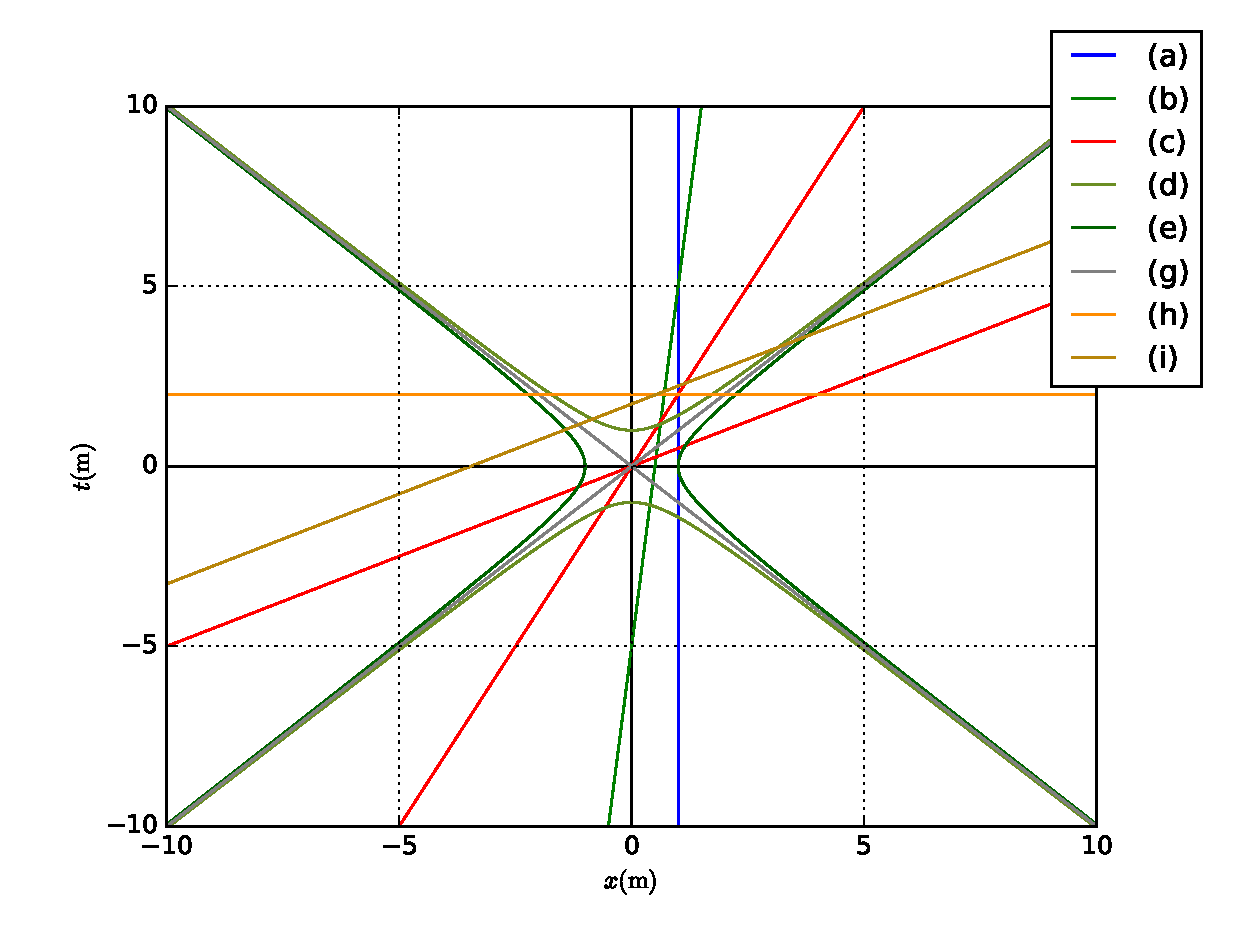
\includegraphics[width=0.95\textwidth]{img/problem_3}

  \caption*{Exercise 3}
\end{figure}


\textbf{4}
Write out all the terms of the following sums, substituting the coordinate names $(t, x, y, z)$ for $(x^0, x^1, x^2, x^3)$:

(a)
$\sum_{\alpha=0}^3 V_\alpha \dd{x^\alpha} =
 V_0 \dd{t} + V_1 \dd{x} + V_2 \dd{y} + V_3 \dd{z}$.

(b)
$\sum_{i=1}^3 (\dd{x^i})^2 =
 \dd{x}^2 + \dd{y}^2 + \dd{z}^2 = \dd{r}^2$.


\textbf{5}

(a) Use the spacetime diagram of an observer $\obs$ to describe the following experiment performed by $\obs$. Two bursts of particles of speed $v = 0.5$ are emitted from $x = 0$ at $t = \SI{-2}{\meter}$, one traveling in the $+x$ direction and the other in the $-x$ direction. These encounter detectors located at $x = \pm\SI{2}{\meter}$. After a delay of $\SI{0.5}{\meter}$ of time, the detectors send signals back to $x = 0$ at speed $v = 0.75$.

\emph{See figure below}


(b) The signals arrive back at $x = 0$ at the same event. (Make sure your spacetime diagram shows this!) From this the experimenter concludes that the particle detectors did indeed send out their signals simultaneously, since he knows they are equal distances from $x = 0$. Explain why this conclusion is valid.

Assuming he knows the signals traveled with equal speeds, and the detectors are an equal distance away, then they must have been emitted simultaneously, in order for them to arrive at $x = 0$ simultaneously.


(c) A second observer $\bar\obs$ moves with speed $v = 0.75$ in the $-x$ direction relative to $\obs$. Draw the spacetime diagram of $\bar\obs$ and in it depict the experiment performed by $\obs$. Does $\bar\obs$ conclude that particle detectors sent out their signals simultaneously? If not, which signal was sent first.

See the diagram below. On it, I have drawn lines $\bar{t}_{\rm left}$ and $\bar{t}_{\rm right}$ (note that they are parallel to the $\bar{x}$ axis). As you can see from the plot, the left emission occurs \emph{before} the right emission.


(d)

Using $\obs$, the distance is
%
\begin{displaymath}
\Delta s^2 = \Delta x^2 = \SI{16}{\meter^2}.
\end{displaymath}
%
Using $\bar\obs$, we first need to find $\bar{x}_{\{a,b\}}$ and $\bar{t}_{\{a,b\}}$. We use the Lorentz transformation to do this.
%
\begin{align*}
  \bar{t} &= \gamma (t - vx)
  \\
  \bar{x} &= \gamma (x - vt)
\end{align*}
%
Using this, we find
\begin{align*}
  \bar{t}_a &= \frac{16 \sqrt7}{7} &
  \bar{t}_b &= \frac{4 \sqrt7}{7}
  \\
  \bar{x}_a &= \frac{-31 \sqrt7}{14} &
  \bar{x}_b &= \frac{\sqrt7}{14}
\end{align*}
%
This gives us a distance of
%
\begin{displaymath}
  \Delta \bar{s}^2 = -(\Delta \bar{t})^2 + (\Delta \bar{x})^2 = \SI{16}{\meter^2},
\end{displaymath}
%
which is of course what we expect.

\begin{figure}[h]
  \centering
  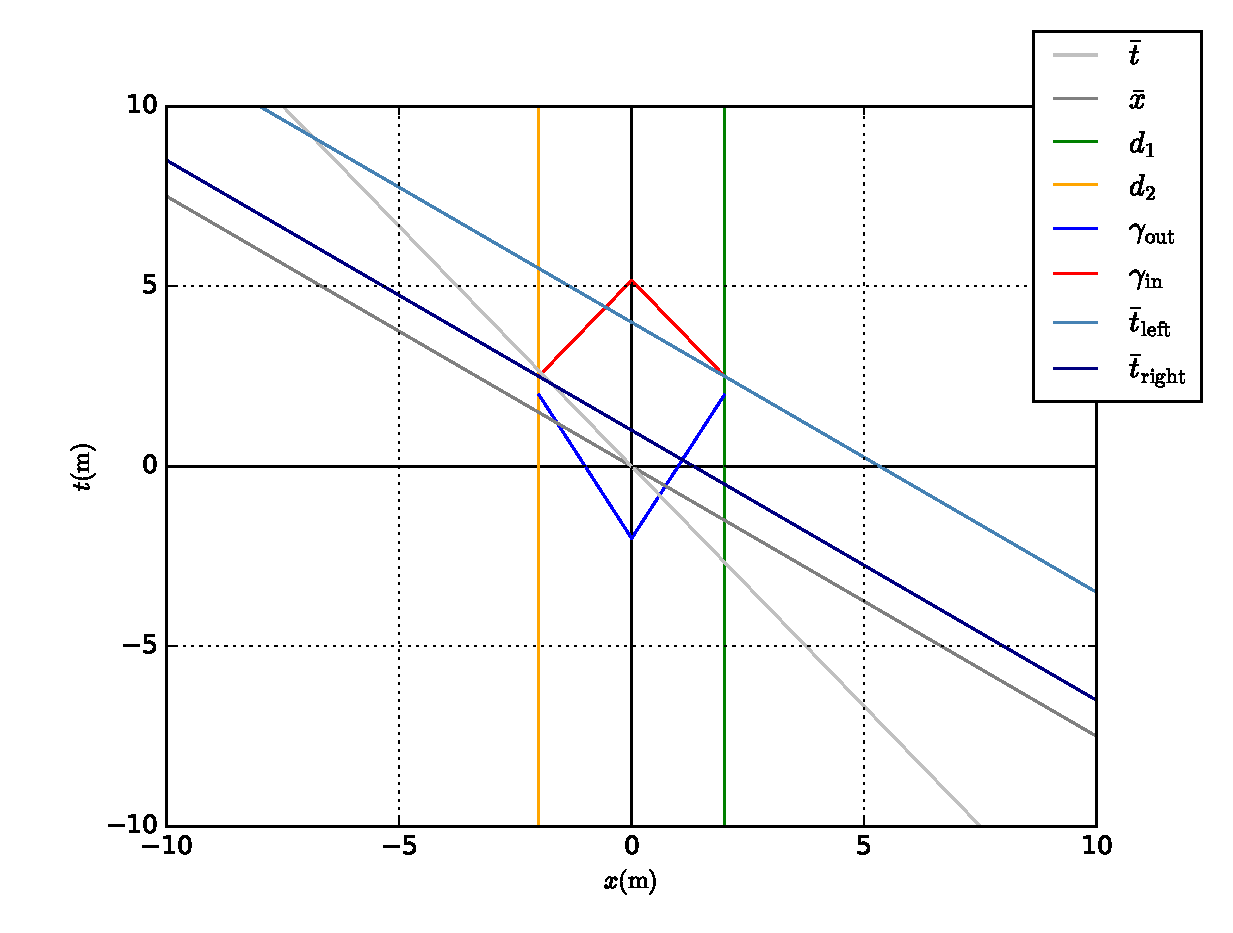
\includegraphics[width=0.95\textwidth]{img/problem_5}

  \caption*{Exercise 5}
\end{figure}


\textbf{6}
Show that Equation (\ref{schutz:1.2}) contains only $M_{\alpha\beta} + M_{\beta\alpha}$ when $\alpha \neq \beta$, not $M_{\alpha\beta}$ and $M_{\beta\alpha}$ independently. Argue that this enables us to set $M_{\alpha\beta} = M_{\beta\alpha}$ without loss of generality.

When we expand the summation in (\ref{schutz:1.2}), there is no point where
%
\begin{displaymath}
  \dd{\bar{s}}^2 =
  \ldots +
  M_{\alpha\alpha} (\dd{x^\alpha})^2 +
  M_{\alpha\alpha} (\dd{x^\alpha})^2 +
  \ldots
\end{displaymath}
occurs, because a double summation only contains $M_{\alpha\alpha}$ once. If it did, we could absorb the two $M_{\alpha\beta}$ terms into a single one. Therefore we can assert the first point.

Now we consider the second point. If we expand the summation, assuming now that an $M_{\alpha\beta}$ and $M_{\beta\alpha}$ term only occur when $\alpha \neq \beta$, then we see
%
\begin{align*}
  \dd{\bar{s}}^2 &=
  \ldots +
  M_{\alpha\beta} (\dd{x^\alpha}) (\dd{x^\beta}) +
  M_{\beta\alpha} (\dd{x^\beta}) (\dd{x^\alpha}) +
  \ldots
  \\ &=
  \ldots +
  (M_{\alpha\beta} + M_{\beta\alpha}) \qty[ (\dd{x^\alpha}) (\dd{x^\beta}) ] +
  \ldots
  \\ &=
  \ldots +
  \mathbf{X} \qty[ (\dd{x^\alpha}) (\dd{x^\beta}) ] +
  \ldots.
\end{align*}
%
Now, what really matters in this summation is the value of $\mathbf{X} = M_{\alpha\beta} + M_{\beta\alpha}$, not the individual values of $M_{\alpha\beta}$ and $M_{\beta\alpha}$. Therefore we can \emph{choose}, without loss of generality, $M_{\alpha\beta} = M_{\beta\alpha} = \mathbf{X}/2$, thereby asserting the second point.


\textbf{7}
In the discussion leading up to Equation (\ref{schutz:1.2}), assume that the coordinates of $\bar{\obs}$ are given as the following linear combinations of those $\obs$:
%
\begin{align*}
  \bar{t} &= \alpha t + \beta x,
  \\
  \bar{x} &= \mu t + \nu x,
  \\
  \bar{y} &= a y,
  \\
  \bar{z} &= b z,
\end{align*}
%
where $\alpha$, $\beta$, $\mu$, $\nu$, $a$, and $b$ may be functions of the velocity $\vec{v}$ of $\bar{\obs}$ relative to $\obs$, but they do not depend on the coordinates. Find the values of $M_{\alpha\beta}$ of Equation (\ref{schutz:1.2}).

\begin{align*}
  \dd{\bar{s}}^2 &=
  -(\dd{\bar{t}})^2 + (\dd{\bar{x}})^2 + (\dd{\bar{y}})^2 + (\dd{\bar{z}})^2
  \\ &=
  -(\alpha \dd{t} + \beta \dd{x})^2
  +(\mu \dd{t} + \nu \dd{x})^2
  +(a \dd{y})^2
  +(b \dd{z})^2
  \\ &=
  -\alpha^2 \dd{t}^2 -
  \alpha\beta \dd{t} \dd{x} -
  \beta^2 \dd{x}^2 +
  \mu^2 \dd{t}^2 +
  \mu \nu \dd{t} \dd{x} +
  \nu^2 \dd{x}^2 +
  a^2 \dd{y}^2 +
  b^2 \dd{z}^2
  \\ &=
  (\mu^2 - \alpha^2) \dd{t}^2 +
  (\mu \nu - \alpha \beta) \dd{t} \dd{x} +
  (\nu^2 - \beta^2) \dd{x}^2 +
  a^2 \dd{y}^2 +
  b^2 \dd{z}^2
  \\
  M_{00} &= \mu^2 - \alpha^2
  \\
  M_{01} &= M_{10} = \frac{\mu \nu - \alpha \beta}{2}
  \\
  M_{11} &= \nu^2 - \beta^2
  \\
  M_{22} &= a^2
  \\
  M_{33} &= b^2,
\end{align*}
and all other $M_{\alpha\beta} = 0$.


\textbf{8}

(a) Derive Equation (\ref{schutz:1.3}) from (\ref{schutz:1.2}) for general $M_{\alpha\beta}$.

Equation (\ref{schutz:1.3}) is just an expansion of the summation in (\ref{schutz:1.2}).

We start by taking out the $\dd{t}^2$ term, which corresponds to $\alpha = \beta = 0$, which gives us
%
\begin{displaymath}
  \dd{\bar{s}}^2 = M_{00} (\dd{t})^2 + \ldots,
\end{displaymath}
%
now we use the equivalence of $\dd{t}$ and $\dd{r}$ to make the substitution
%
\begin{displaymath}
  \dd{\bar{s}}^2 = M_{00} (\dd{r})^2 + \ldots.
\end{displaymath}

For the middle terms, we use the fact that $M_{\alpha\beta} = M_{\beta\alpha}$, and look at only the terms where \emph{one} of $\alpha$ and $\beta$ is zero. The symmetry means we can write $M_{0i} = M_{i0}$, and pull out a 2 because there are twice as many terms, giving us
%
\begin{align*}
  \dd{\bar{s}}^2 &=
  M_{00} (\dd{r})^2
  \\ &+
  2 \qty( \sum_{i=1}^3 M_{0i} (\dd{x^i}) (\dd{t}) )
  \\ &+
  \ldots.
\end{align*}
%
Now we use the equivalence of $\dd{t}$ and $\dd{r}$ once again, and pull the term out of the sum, giving us
%
\begin{align*}
  \dd{\bar{s}}^2 &=
  M_{00} (\dd{r})^2
  \\ &+
  2 \qty( \sum_{i=1}^3 M_{0i} \dd{x^i} ) \dd{r}
  \\ &+
  \ldots.
\end{align*}

Finally, we simply include the terms which have not yet been accounted for, which are all the \emph{spacial-only} terms, which arrives us back at Equation (\ref{schutz:1.3}):
%
\begin{align*}
  \dd{\bar{s}}^2 &=
  M_{00} (\dd{r})^2
  \\ &+
  2 \qty( \sum_{i=1}^3 M_{0i} \dd{x^i} ) \dd{r}
  \\ &+
  \sum_{i=1}^3 \sum_{j=1}^3 M_{ij} \dd{x^i} \dd{x^j}.
\end{align*}


(b) Since $\dd{\bar{s}}^2 = 0$ in Equation (\ref{schutz:1.3}), for \emph{any} $\dd{x^i}$, replace $\dd{x^i}$ with $-\dd{x^i}$, and subtract that result from the original equation. This will establish that $M_{0i} = 0$.
%
\begin{align*}
  \dd{\bar{s}}^2 &=
  M_{00} (\dd{r})^2
  \\ &-
  2 \qty( \sum_{i=1}^3 M_{0i} \dd{x^i} ) \dd{r}
  \\ &+
  \sum_{i=1}^3 \sum_{j=1}^3 M_{ij} \dd{x^i} \dd{x^j}.
\end{align*}
%
\begin{align*}
  \dd{\bar{s}}^2 - \dd{\bar{s}}^2 = 0 &=
  \cancel{0 \, M_{00} (\dd{r})^2}
  \\ &+
  4 \qty( \sum_{i=1}^3 M_{0i} \dd{x^i} ) \dd{r}
  \\ &+
  \cancel{0 \sum_{i=1}^3 \sum_{j=1}^3 M_{ij} \dd{x^i} \dd{x^j}}.
\end{align*}
%
\begin{displaymath}
  0 = \cancel{4} \qty( \sum_{i=1}^3 M_{0i} \dd{x^i} ) \cancel{\dd{r}}
\end{displaymath}
%
Now there are two possibilities. In one case, $\dd{x^i} \equiv 0$, but that is a trivial solution and in general is not true. The other case is that $M_{0i} \equiv 0$, which means we can simplify Equation (\ref{schutz:1.3}) to
%
\begin{align*}
  \dd{\bar{s}}^2 &=
  M_{00} (\dd{r})^2
  \\ &+
  \sum_{i=1}^3 \sum_{j=1}^3 M_{ij} \dd{x^i} \dd{x^j}.
\end{align*}


(c) Use the result of part (b) with $\dd{\bar{s}}^2 = 0$ to establish Equation (\ref{schutz:1.4b}).
%
\begin{align*}
  \dd{\bar{s}}^2 = 0 &=
  M_{00} (\dd{r})^2 + \sum_{i=1}^3 \sum_{j=1}^3 M_{ij} \dd{x^i} \dd{x^j}
  \\ \implies
  -M_{00} (\dd{r})^2 &=
  \sum_{i=1}^3 \sum_{j=1}^3 M_{ij} \dd{x^i} \dd{x^j},
\end{align*}
%
now if we expand $(\dd{r})^2$, we see that there can only be non-zero $M_{ij}$ when $i = j$, and so
%
\begin{align*}
  -M_{00} \qty( (\dd{x}^2) + (\dd{y}^2) + (\dd{z}^2) ) &=
  \sum_{i=1}^3 M_{ii} (\dd{x^i})^2
  \\ \implies
  -(M_{00}) \delta_{ij} &=
  M_{ij},
\end{align*}
%
which is simply Equation (\ref{schutz:1.4b}).



\textbf{9}
Explain why the line $\mathcal{P}\mathcal{L}$ in Figure 1.7 is drawn in the manner described in the text.

% The key here is that both $\mathcal{P}$ and $\mathcal{L}$ must emit or absorb a beam of light, which intersect the same reflection points at $\mathcal{A}$ and $\mathcal{B}$. This means that they occur at $t = \bar{t} = 0$. This also means that from $\bar{\obs}$, it appears that the light reflected from



\textbf{10}
For the pairs of events whose coordinates $(t,x,y,z)$ in some frame are given below, classify their separations as timelike, spacelike, or null.

(a) $(0,0,0,0)$ and $(-1,1,0,0)$:
\begin{displaymath}
  \dd{s}^2 =
  -(0 + 1)^2 + (0 - 1)^2 + (0 - 0)^2 + (0 - 0)^2 =
  -1 + 1 + 0 + 0 =
  0 \implies
  \mathrm{null}
\end{displaymath}

(b) $(1,1,-1,0)$ and $(-1,1,0,2)$:
\begin{displaymath}
  \dd{s}^2 =
  -(1 + 1)^2 + (1 - 1)^2 + (-1 - 0)^2 + (0 - 2)^2 =
  -4 + 0 + 1 + 4 =
  1 \implies
  \mathrm{spacelike}
\end{displaymath}

(c) $(6,0,1,0)$ and $(5,0,1,0)$:
\begin{displaymath}
  \dd{s}^2 =
  -(6 - 5)^2 + (0 - 0)^2 + (1 - 1)^2 + (0 - 0)^2 =
  -1 + 0 + 0 + 0 =
  -1 \implies
  \mathrm{timelike}
\end{displaymath}

(d) $(-1,1,-1,1)$ and $(4,1,-1,6)$:
\begin{displaymath}
  \dd{s}^2 =
  -(-1 - 4)^2 + (1 - 1)^2 + (-1 + 1)^2 + (1 - 6)^2 =
  -25 + 0 + 0 + 25 =
  0 \implies
  \mathrm{null}
\end{displaymath}


\textbf{11}
Show that the hyperbolae $-t^2 + x^2 = a^2$ and $-t^2 + x^2 = -b^2$ are asymptotic to the lines $t = \pm x$, regardless of $a$ and $b$.

We will generalize $a$ and $-b$ with a new constant, $\alpha \in \mathbb{R}$, and so we have: $-t^2 + x^2 = \alpha^2$. Now if we solve for $t$, we get $t = \pm \sqrt{x^2 - \alpha^2}$.

Now take the limit of $t$ as $x \to \infty$ (or $-\infty$, they are equivalent since $x$ is real and squared), which gives us:
\begin{align*}
  \lim_{x\to\infty} t &=
  \lim_{x\to\infty} \pm \sqrt{x^2 - \alpha^2} =
  \pm \sqrt{x^2} = \pm x.
\end{align*}

Note that we dropped the $\alpha^2$ term in the limit, as it was being subtracted from a number approaching infinity, and was therefore negligible.


\textbf{12}

(a) Use the fact that the tangent to the hyperbola $\mathcal{DB}$ in Figure 1.14 is the line of simultaneity for $\bar\obs$ to show that the time interval $\mathcal{AE}$ is shorter than the time recorded on $\bar\obs$'s clock as it moved from $\mathcal{A}$ to $\mathcal{B}$.

If we look at the figure, we see that $\mathcal{AD}$ and $\mathcal{AB}$ lie along the same hyperbola. This means that when $\obs$ measures $\dd{t} = \mathcal{AD}$, and $\bar\obs$ measures $\dd{\bar{t}} = \mathcal{AB}$, the two measurements are the same. Since $\dd{t} = \mathcal{AE}$ is clearly shorter than $\dd{t} = \mathcal{AD}$, then $\dd{t} = \mathcal{AD} < \dd{\bar{t}} = \mathcal{AB}$.


(b) Calculate that
%
\begin{displaymath}
  (\dd{s}^2)_{\mathcal{AC}} =
  (1 - v^2) (\dd{s}^2)_{\mathcal{AB}}
\end{displaymath}
%
\begin{align*}
  (\dd{s}^2)_{\mathcal{AC}} &=
  -(\dd{t})_{\mathcal{AC}}^2
  \\
  (\dd{s}^2)_{\mathcal{AB}} &=
  (\dd{\bar{s}}^2)_{\mathcal{AB}}
  \\ &=
  -(\dd{\bar{t}})_{\mathcal{AB}}^2
  \\ &=
  -(\gamma (\dd{t} - v \dd{x}))^2 =
  -(\gamma (\dd{t} - v \cdot 0))^2 =
  -(\gamma \dd{t})^2 =
  \gamma^2 [-(\dd{t})^2]
  \\ &=
  \gamma^2 (\dd{s}^2)_{\mathcal{AC}} =
  \frac{(\dd{s}^2)_{\mathcal{AC}}}{1 - v^2}
  \\ \implies
  (\dd{s}^2)_{\mathcal{AC}} &=
  (1 - v^2) (\dd{s}^2)_{\mathcal{AB}}
\end{align*}


\textbf{13}
The Half-life of the elementary particle called the $\pi$-meson (or pion) is $\SI{2.5e-8}{\second}$ when the pion is at rest relative to the observer measuring its decay time. Show, by the principle of relativity, that pions moving at speed $v = 0.999$ must have a half-life of $\SI{5.6e-7}{\second}$, as measured by an observer at rest.
%
\begin{displaymath}
  \dd{t} =
  \gamma \dd{\bar{t}} =
  \frac{\SI{2.5e-8}{\second}}{\sqrt{1 - 0.999^2}} \approx
  \SI{5.59e-7}{\second}
\end{displaymath}



\textbf{14}
Suppose the velocity $\vb{v}$ of $\bar\obs$ relative to $\obs$ is small, $\abs{\vb{v}} \ll 1$. Show that the time dilation, Lorentz contraction, and velocity-addition formulae can be approximated by respectively:

(a) $\dd{t} \approx (1 + \frac{1}{2} v^2) \dd{\bar{t}}$

\begin{align*}
  \gamma &=
  (1 - v^2)^{-1/2} =
  \sum_{k=0}^\infty \binom{-1/2}{k} x^k =
  1 + (-1/2) (-v^2) + \frac{(-1/2) (-1/2 - 1)}{2!} (-v^2)^2 + \ldots \approx
  1 + \frac{1}{2} v^2
  \\
  \dd{t} &=
  \gamma \dd{\bar{t}} \approx
  \qty(1 + \frac{1}{2} v^2) \dd{\bar{t}}
\end{align*}

(b) $\dd{x} \approx (1 - \frac{1}{2} v^2) \dd{\bar{x}}$

\begin{align*}
  \gamma^{-1} &=
  (1 - v^2)^{1/2} =
  \sum_{k=0}^\infty \binom{1/2}{k} x^k =
  1 + (1/2) (-v^2) + \frac{(1/2) (1/2 - 1)}{2!} (-v^2)^2 + \ldots \approx
  1 - \frac{1}{2} v^2
  \\
  \dd{x} &=
  \gamma^{-1} \dd{\bar{x}} \approx
  \qty(1 - \frac{1}{2} v^2) \dd{\bar{x}}
\end{align*}


(c) $W' \approx W + v - W v (W + v)$ (with $\abs{W} \ll 1$ as well)

\begin{align*}
  W' &=
  \frac{W + v}{1 + W v} =
  (W + v) (1 + W v)^{-1}
  \\
  (1 + W v)^{-1} &=
  \sum_{k=0}^\infty \binom{-1}{k} (W v)^k =
  1 -
  W v +
  \frac{1}{2} \cdot 1 (1 + 1) (W v)^2 -
  \frac{1}{6} \cdot 1 (1 + 1) (1 + 2) (W v)^3 + \ldots
  \\ &\approx
  1 - W v + (W v)^2
  \\
  W' &\approx
  (W + v) (1 - W v + (W v)^2) =
  W + v - W v (W + v) + (W v)^2 (W + v)
  \\ &\approx
  W + v - W v (W + v)
\end{align*}

What are the relative errors in these approximations when $\abs{\vb{v}} = W = 0.1$?

\textbf{TODO}


\textbf{15}
Suppose that the velocity $\vb{v}$ of $\bar\obs$ relative to $\obs$ is nearly that of light, $\abs{\vb{v}} = 1 - \varepsilon$, $0 < \varepsilon \ll 1$. Show that the same formulae of Exercise 14 become

(a) $\dd{t} \approx \dd{\bar{t}} / \sqrt{2 \varepsilon}$

\begin{align*}
  v &=
  1 - \varepsilon \implies
  v^2 = (1 - \varepsilon)^2 =
  1 - 2 \varepsilon + \varepsilon^2
  \\ \implies
  1 - v^2 &=
  1 - (1 - 2 \varepsilon + \varepsilon^2) =
  2 \varepsilon - \varepsilon^2 =
  2 \varepsilon \qty(1 - \frac{\varepsilon}{2})
  \\
  \gamma &=
  (1 - v^2)^{-1/2} =
  \qty(2 \varepsilon \qty(1 - \frac{\varepsilon}{2}))^{-1/2} =
  \frac{1}{\sqrt{2 \varepsilon}} \qty(1 - \frac{\varepsilon}{2})^{-1/2} \approx
  \frac{1}{\sqrt{2 \varepsilon}}
  \\
  \dd{t} &=
  \gamma \dd{\bar{t}} \approx
  \frac{\dd{\bar{t}}}{\sqrt{2 \varepsilon}}
\end{align*}

(b) $\dd{x} \approx \dd{\bar{x}} \sqrt{2 \varepsilon}$

\begin{align*}
  v &=
  1 - \varepsilon \implies
  v^2 = (1 - \varepsilon)^2 =
  1 - 2 \varepsilon + \varepsilon^2
  \\ \implies
  1 - v^2 &=
  1 - (1 - 2 \varepsilon + \varepsilon^2) =
  2 \varepsilon - \varepsilon^2 =
  2 \varepsilon \qty(1 - \frac{\varepsilon}{2})
  \\
  \gamma^{-1/2} &=
  (1 - v^2)^{1/2} =
  \qty(2 \varepsilon \qty(1 - \frac{\varepsilon}{2}))^{1/2} =
  \sqrt{2 \varepsilon} \qty(1 - \frac{\varepsilon}{2})^{1/2} \approx
  \sqrt{2 \varepsilon}
  \\
  \dd{x} &=
  \gamma^{-1} \dd{\bar{x}} \approx
  \dd{\bar{t}} \sqrt{2 \varepsilon}
\end{align*}

(c) $W' \approx 1 - \varepsilon (1 - W) / (1 + W)$

\textbf{TODO}

What are the relative errors on these approximations when $\varepsilon = 0.1$ and $W = 0.9$?

\textbf{TODO}


\textbf{16}
Use the Lorentz transformation, Equation 1.12, to derive (a) the time dilation, and (b) the Lorentz contraction formulae. Do this by identifying pairs of events where the separations (in time or space) are to be compared, and then using the Lorentz transformation to accomplish the algebra that the invariant hyperb b olae had been used for in the text.

(a)
To derive the time dilation formula, we choose two events that occur at $x = c$, and times $t_1$ and $t_2$. Thus, from $\obs$'s frame, the time elapsed between these two events is $\Delta t = t_2 - t_1$, and the distance between them is $\Delta x = 0$. Another observer, $\bar\obs$, moves with some velocity $v$ relative to $\obs$. As it passes through the lines $t = t_1$ and $t = t_2$, its clock moves forward by a time $\Delta \tau = \bar{t}_2 - \bar{t}_1$. We now use the Lorentz transformation to write $\Delta \tau$ in terms of $\obs$'s coordinates.
%
\begin{align*}
  \Delta \tau &=
  \bar{t}_2 - \bar{t}_1 =
  \gamma \qty[ (t_2 - v x_2) - (t_1 - v x_1) ] =
  \gamma \qty[ (t_2 - t_1) + (v x_1 - v x_2) ]
  \\ &=
  \gamma \qty[ \Delta t + v \Delta x ] =
  \gamma \qty[ \Delta t + v \cdot 0 ]
  \\ &=
  \gamma \Delta t
\end{align*}
%
and thus we have arrived at the formula for time dilation.

(b)
To derive the Lorentz contraction formula, we take a slightly different approach. In the $\obs$ frame, a stick lies parallel to $x$, such that its length $\ell = x_2 - x_1$. In this frame, the world lines of the two ends of the stick form vertical lines. Another observer, $\bar\obs$, moves with a velocity $v$, relative to $\obs$. Two events, $\mathcal{A}$ and $\mathcal{B}$ occur on either end of the stick, such that $\bar\obs$ observes the two events to be simultaneous. Thus, from the $\bar\obs$ frame, the events are located a distance $\Delta \bar{x} = \bar{\ell}$ apart, and $\Delta \bar{t} = 0$. However, from the $\obs$ frame, the events occur a distance $\Delta x = \ell$ apart, and a time separation $\Delta t \neq 0$.
%
\begin{align*}
  \ell &=
  x_2 - x_1 =
  \gamma \qty[ (\bar{x}_2 - v \bar{t}_2) - (\bar{x}_1 - v \bar{t}_1) ] =
  \gamma \qty[ (\bar{x}_2 - \bar{x}_1) + v (\bar{t}_1 - \bar{t}_2) ] =
  \gamma \bar{\ell}
  \\ \implies
  \bar{\ell} = \frac{\ell}{\gamma}
\end{align*}


\textbf{17}
A lightweight pole, $\SI{20}{\meter}$ long, lies on the ground next to a barn $\SI{15}{\meter}$ long. An Olympic athlete picks up the pole, carries it far away, and runs with it toward the end of the barn at a speed $0.8$. His friend remains at rest, standing by the door of the barn. Attempt all parts of this question, even if you can't answer some.

(a) How long does the friend measure the pole to be, as it approaches the barn?

We use the Lorentz contraction equation to find the length the friend measures.
%
\begin{align*}
  \bar\ell &=
  \ell / \gamma =
  \ell \sqrt{ 1 - v^2 } =
  \SI{20}{\meter} \sqrt{ 1 - 0.8^2 } =
  \SI{12}{\meter}
\end{align*}

(b) The barn door is initially open and, immediately after the runner and pole are entirely inside the barn, the friend shuts the door. How long after the door is shut does the front of the pole hit the other end of the barn, as measured by the friend? Compute the interval between the events of shutting the door and hitting the wall. Is it spacelike, timelike, or null?

From the runner's point of view, we must consider the length contraction of the barn

(c) In the reference frame of the runner, what is the length of the barn and the pole?


(d) Does the runner believe that the pole is entirely inside the barn when its front hits the end of the barn? Can you explain why?


(e) After the collision, the pole and runner come to rest relative to the barn. From the friend's point of view, the $\SI{20}{\meter}$ pole is now inside a $\SI{15}{\meter}$ barn, since the barn door was shut before the pole stopped. How is this possible? Alternatively, from the runner's point of view, the collision should have stopped the pole \emph{before} the door closed, so the door could not be closed at all. Was or was not the door closed with the pole inside?


(f) Draw a spacetime diagram from the friend's point of view and use it to illustrate and justify all your conclusions.




\textbf{18}

(a) The Einstein velocity-addition law, Equation 1.13, has a simpler form if we introduce the concept of the \emph{velocity parameter} $u$, defined by the equation
%
\begin{displaymath}
  v = \tanh u.
\end{displaymath}
%
Notice that for $-\infty < u < \infty$, the velocity is confined to the acceptable limits $-1 < v < 1$. Show that if
%
\begin{displaymath}
  v = \tanh u
\end{displaymath}
%
and
%
\begin{displaymath}
  w = \tanh U,
\end{displaymath}
%
then Equation 1.13 implies
%
\begin{displaymath}
  w' = \tanh(u + U).
\end{displaymath}
%
This means that velocity parameters add linearly.

There exists an identity:
%
\begin{displaymath}
  \tanh(x+y) = \frac{\tanh(x) + \tanh(y)}{1 + \tanh(x) \tanh(y)}.
\end{displaymath}
%
If we simply use $x=u$ and $y=U$, then we arrive at
%
\begin{displaymath}
  \tanh(u+U) = \frac{\tanh(u) + \tanh(U)}{1 + \tanh(u) \tanh(U)} = w'
\end{displaymath}


(b) Use this to solve the following problem. A star measures a second star to be moving away at speed $v = 0.9$. The second star measures a third to be receding in the same direction at $0.9$. Similarly, the third measures a fourth, and so on, up to some large number $N$ of stars. What is the velocity of the $N$th star relative to the first? Give an exact answer and an approximation useful for large $N$.

Let $w^N$ be the velocity of the $N$th star relative to the original star, which we will call star $0$. We will use an induction proof to find an expression for $w^N$. The base case is trivial, $w^0 = 0$, as the star does not move relative to itself. For the next case, $w^1 = v$, we still aren't really doing velocity addition, so we will skip to the $w^2$ case, where things get interesting, though we will later show that the general expression holds for $w^0$ and $w^1$.

For $w^2$, we simply use the Einstein velocity-addition law:
%
\begin{displaymath}
  w^2 =
  \tanh(u + U) =
  \tanh(\tanh^{-1} v + \tanh^{-1} w^1) =
  \tanh(2 \tanh^{-1} v).
\end{displaymath}
%
Now I will prove that this is one instance of a general expression, that $w^N = \tanh(N \tanh^{-1} v)$.
%
\begin{align*}
  & w^N =
  \tanh(N \tanh^{-1} v)
  \\ \implies &
  \tanh^{-1} w^N =
  N \tanh^{-1} v
  \\ \implies &
  \tanh^{-1} w^N + \tanh^{-1} v =
  N \tanh^{-1} v + \tanh^{-1} v
  \\ \implies &
  \tanh^{-1} w^N + \tanh^{-1} v =
  (N+1) \tanh^{-1} v
  \\ \implies &
  \tanh( \tanh^{-1} w^N + \tanh^{-1} v ) =
  \tanh( (N+1) \tanh^{-1} v )
  \\ \implies &
  w^{N+1} =
  \tanh( (N+1) \tanh^{-1} v ).
\end{align*}
%
If you can believe the last step, then this is proof that it works for all $N$. The last step is saying that, if we have a star $N$, moving away from star $0$ at a speed $w^N$, and another star $N+1$, moving away from star $N$ at a speed $v$, then star $N+1$ as observed from star $0$ is given by the Einstein velocity-addition law, meaning we can rewrite that expression as $w^{N+1}$.

Now I'd like to go back and show that this works for $N=0$ and $N=1$. For $N=1$, we get
%
\begin{displaymath}
  w^1 = \tanh( 1 \tanh^{-1} v ) = v,
\end{displaymath}
%
which is what we would expect, and for $N=0$, we get
%
\begin{displaymath}
  w^0 = \tanh( 0 \tanh^{-1} v ) = 0,
\end{displaymath}
%
which we also expect. So the general expression,
%
\begin{displaymath}
  w^N = \tanh( N \tanh^{-1} v ),
\end{displaymath}
%
holds true for all non-negative integers $N$. We can also write this more elegantly as
%
\begin{displaymath}
  w^N = \tanh( N u ).
\end{displaymath}

Now we want to consider the behaviour at large $N$. We first write $\tanh$ in its exponential form, as
%
\begin{displaymath}
  w^N = \frac{1 - \exp(-2 N u)}{1 + \exp(-2 N u)}.
\end{displaymath}
%
When $N$ is very large, then the exponential in the bottom term goes to zero, allowing us to rewrite it as
%
\begin{displaymath}
  w^N \approx 1 - \exp(-2 N u).
\end{displaymath}
%
We can go a step further. Since $v = 0.9$, $u \approx 1.47$, which we can neglect for large $N$, and so we finally arrive at
%
\begin{displaymath}
  w^N \approx 1 - \exp(-2 N).
\end{displaymath}


\textbf{19}

(a) Using the velocity parameter ($u$) introduced in Exercise 18, show that the Lorentz transformation equations, Equation 1.12, can be put in the form
%
\begin{align*}
  \bar{t} &=  t \cosh u - x \sinh u & \bar{y} &= y
  \\
  \bar{x} &= -t \sinh u + x \cosh u & \bar{z} &= z
\end{align*}

We start by putting $\gamma$ in terms of $u$.
%
\begin{align*}
  \gamma &=
  (1 - v^2)^{-1/2} =
  (1 - \tanh^2 u)^{-1/2} =
  \frac{1}{\sech u} =
  \cosh u.
\end{align*}
%
Now we can substitute this into the Lorentz transformation equations
%
\begin{align*}
  \bar{t} &=
  \gamma (t - v x) =
  \cosh u (t - x \tanh u) =
  t \cosh u - x \sinh u
  \\
  \bar{x} &=
  \gamma (x - v t) =
  \cosh u (x - t \tanh u) =
  x \cosh u - t \sinh u
\end{align*}

(b) Use the identity $\cosh^2 u - \sinh^2 u = 1$ to demonstrate the invariance of the interval from these equations.
%
\begin{align*}
  \dd{s}^2 &= -\dd{t}^2 + \dd{x}^2 + \dd{y}^2 + \dd{z}^2
  \\
  \dd{\bar{s}}^2 &=
  -\qty(\dd{t} \cosh u - \dd{x} \sinh u)^2
  +\qty(\dd{x} \cosh u - \dd{t} \sinh u)^2
  + \dd{y}^2 + \dd{z}^2
  \\ &=
  -\qty(\dd{t}^2 \cosh^2 u -
        \cancel{\dd{x} \dd{t} \sinh u \cosh u} +
        \dd{x}^2 \sinh^2 u)
  \\ &+
  \qty(\dd{x}^2 \cosh^2 u -
        \cancel{\dd{t} \dd{x} \sinh u \cosh u} +
        \dd{t}^2 \sinh^2 u)
  + \dd{y}^2 + \dd{z}^2
  \\ &=
  -\dd{t}^2 \cancel{\qty(\cosh^2 u - \sinh^2 u)} +
  \dd{x}^2 \cancel{\qty(\cosh^2 u - \sinh^2 u)}
  + \dd{y}^2 + \dd{z}^2
  \\ &=
  \dd{s}^2
\end{align*}

(c) Draw as many parallels as you can between the geometry of spacetime and ordinary two-dimensional Euclidean geometry, where the coordinate transformation analogous to the Lorentz transformation is
%
\begin{align*}
  \bar{x} &= +x \cos\theta + y \sin\theta,
  \\
  \bar{y} &= -x \sin\theta + y \cos\theta.
\end{align*}
%
What is the analog of the interval? Of the invariant hyperbolae?

The analog of the interval would be
%
\begin{align*}
  \dd{\bar{r}}^2 &=
  \dd{\bar{x}}^2 + \dd{\bar{y}}^2 =
  (\dd{x} \cos\theta + \dd{y} \sin\theta)^2 +
  (\dd{y} \cos\theta - \dd{x} \sin\theta)^2 +
  \\ &=
  \dd{x}^2 \cos^2 \theta +
  \cancel{2 \dd{x} \dd{y} \sin\theta \cos\theta} +
  \dd{y}^2 \sin^2 \theta
  \\ &+
  \dd{y}^2 \cos^2 \theta -
  \cancel{2 \dd{x} \dd{y} \sin\theta \cos\theta} +
  \dd{x}^2 \sin^2 \theta
  \\ &=
  \dd{x}^2 (\sin^2 \theta + \cos^2 \theta) +
  \dd{y}^2 (\sin^2 \theta + \cos^2 \theta)
  \\ &=
  \dd{x}^2 + \dd{y}^2
\end{align*}
%
The analog of the invariant hyperbola would be the invariant circle, as $\bar{x}$ and $\bar{y}$ are both equations of a circle.


\textbf{20}
Write the Lorentz transformation equations in matrix form.

\begin{align*}
  \bar{t} &= \gamma (t - v x) &
  \bar{t} &= \gamma t - \gamma v x + 0 y + 0 z
  \\
  \bar{x} &=  \gamma (x - v t) &
  \bar{x} &= -\gamma v t + \gamma x + 0 y + 0 z
  \\
  \bar{y} &= y & \bar{y} &= y
  \\
  \bar{z} &= z & \bar{z} &= z
  \\
  \mqty( \bar{t} \\ \bar{x} \\ \bar{y} \\ \bar{z} ) &=
  \mqty( \gamma   & -\gamma v & 0 & 0 \\
        -\gamma v &  \gamma   & 0 & 0 \\
         0        &  0        & 1 & 0 \\
         0        &  0        & 0 & 1 )
  \mqty( t \\ x \\ y \\ z )
\end{align*}


\textbf{21}

(a) Show that if the two events are timelike separated, there is a Lorentz frame in which they occur at the same point, i.e. at the same spatial coordinate values.

If the two events are timelike separated, then it must be possible to have an object with a worldline which crosses the two points, as it is inside the light cone. If such an object exists, then we can draw a Lorentz frame for it, so its time axis, $\bar{t}$ is that line, meaning $\bar{x} = 0$ for both events.


(b) Similarly, if the two events are spacelike separated, there is a Lorentz frame in which they occur simultaneously.

If the two events are spacelike separated, then it must be possible to draw a coordinate frame where $\bar{x}$ has slope $v$ in $\obs$'s frame. This means that $\bar{t} = 0$ for both events, and so they are simultaneous.



\end{document}